\documentclass[8pt,a4paper]{article}
\usepackage{graphicx}
\usepackage{amsmath}
\usepackage{amsfonts}
\usepackage{amssymb,amsthm}
\usepackage{array}
\usepackage[utf8]{inputenc} 

 
\begin{document}
%style file for ESANN manuscripts
\title{Procesamiento de texto manuscrito usando conjuntos de clasificadores}

%***********************************************************************
% AUTHORS INFORMATION AREA
%***********************************************************************
\author{
Emilio Samuel Aced Fuentes \\
Roberto Alcober Couso \\
Arturo Bl\'azquez P\'erez \\
Nicol\'as Trejo Moya \\
}
%***********************************************************************
% END OF AUTHORS INFORMATION AREA
%***********************************************************************

\maketitle

\section{Introducci\'on}
En este proyecto vamos a clasificar im\'agenes de letras manuscritas intentando predecir de forma correcta el s\'imbolo que representan.
Utilizaremos varios algoritmos de clasificaci\'on y los compararemos para encontrar los mejores resultados posibles, viendo diferencias de tiempos y  tasa de acierto.


\section{An\'alisis de los datos}
En el dataset provisto, est\'an representadaslas 10 primeras letras del alfabeto(A-J), por tanto 10 clases las cuales hemos etiquetado en nuestra base de datos etiquetadas de 0 a 10 respectivamente.
Las imagenes nos vienen en un tamaño de $206\times150$ en escala de grises.
 
\begin{figure}[htbp]
	\centering
    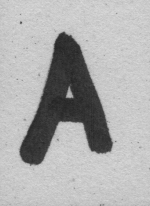
\includegraphics[scale=0.5]{./sin_procesar/l00000_A.png}
    \caption{Ejemplo de una A}
\end{figure}
 
There's a picture of a galaxy above
\end{document}